\subsection{Покадровое детектирование}

В начале работы над этапом детектирования было запущено обучение модели YOLOv5m на датасете VisDrone длительностью в 50 эпох, результатом которого стал $mAP \ 30.0$, в связи с чем был проведен анализ плохо детектируемых объектов, которыми оказались малопредставленные в датасете классы, такие как bus, tricycle и truck, что следует из Рис. \ref{img:10-1} и \ref{img:10-2}, а также объекты малого размера, в частности, в плотных группах на заднем плане.

\vspace{0.5cm}

\begin{figure}[ht]
    \centering
    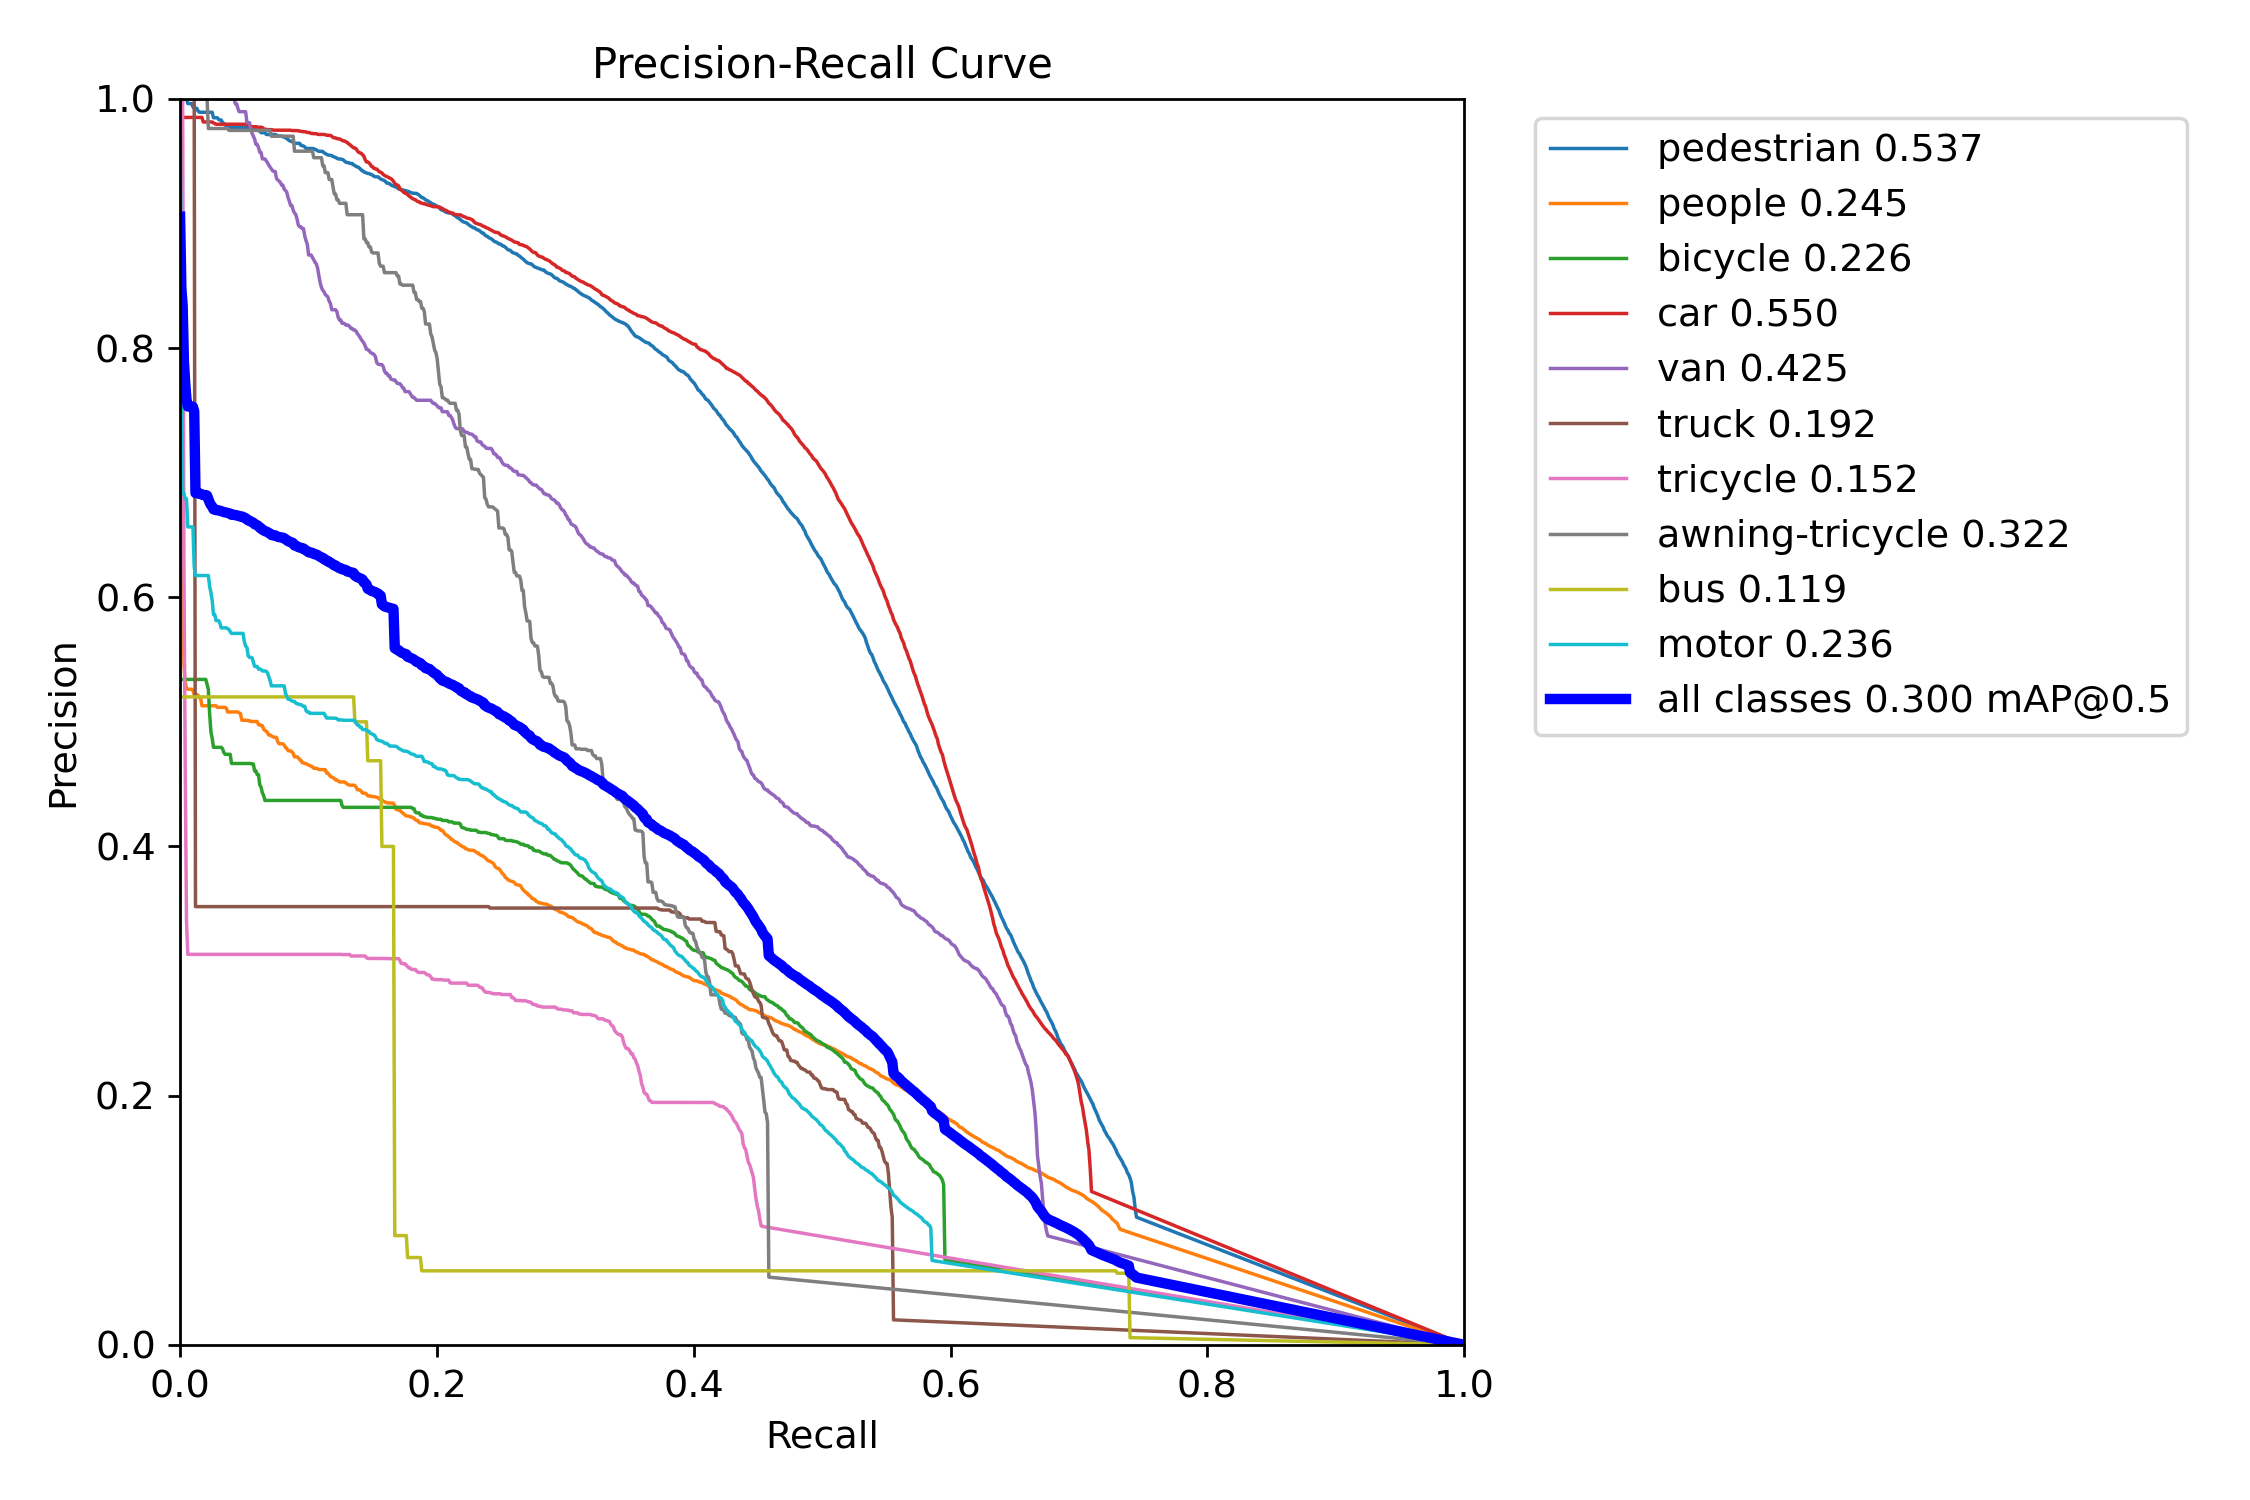
\includegraphics[width=0.85\textwidth]{10-1}
    \caption{Precision-Recall Curve после первого этапа обучения}
    \label{img:10-1}
\end{figure}

\begin{figure}[ht]
    \centering
    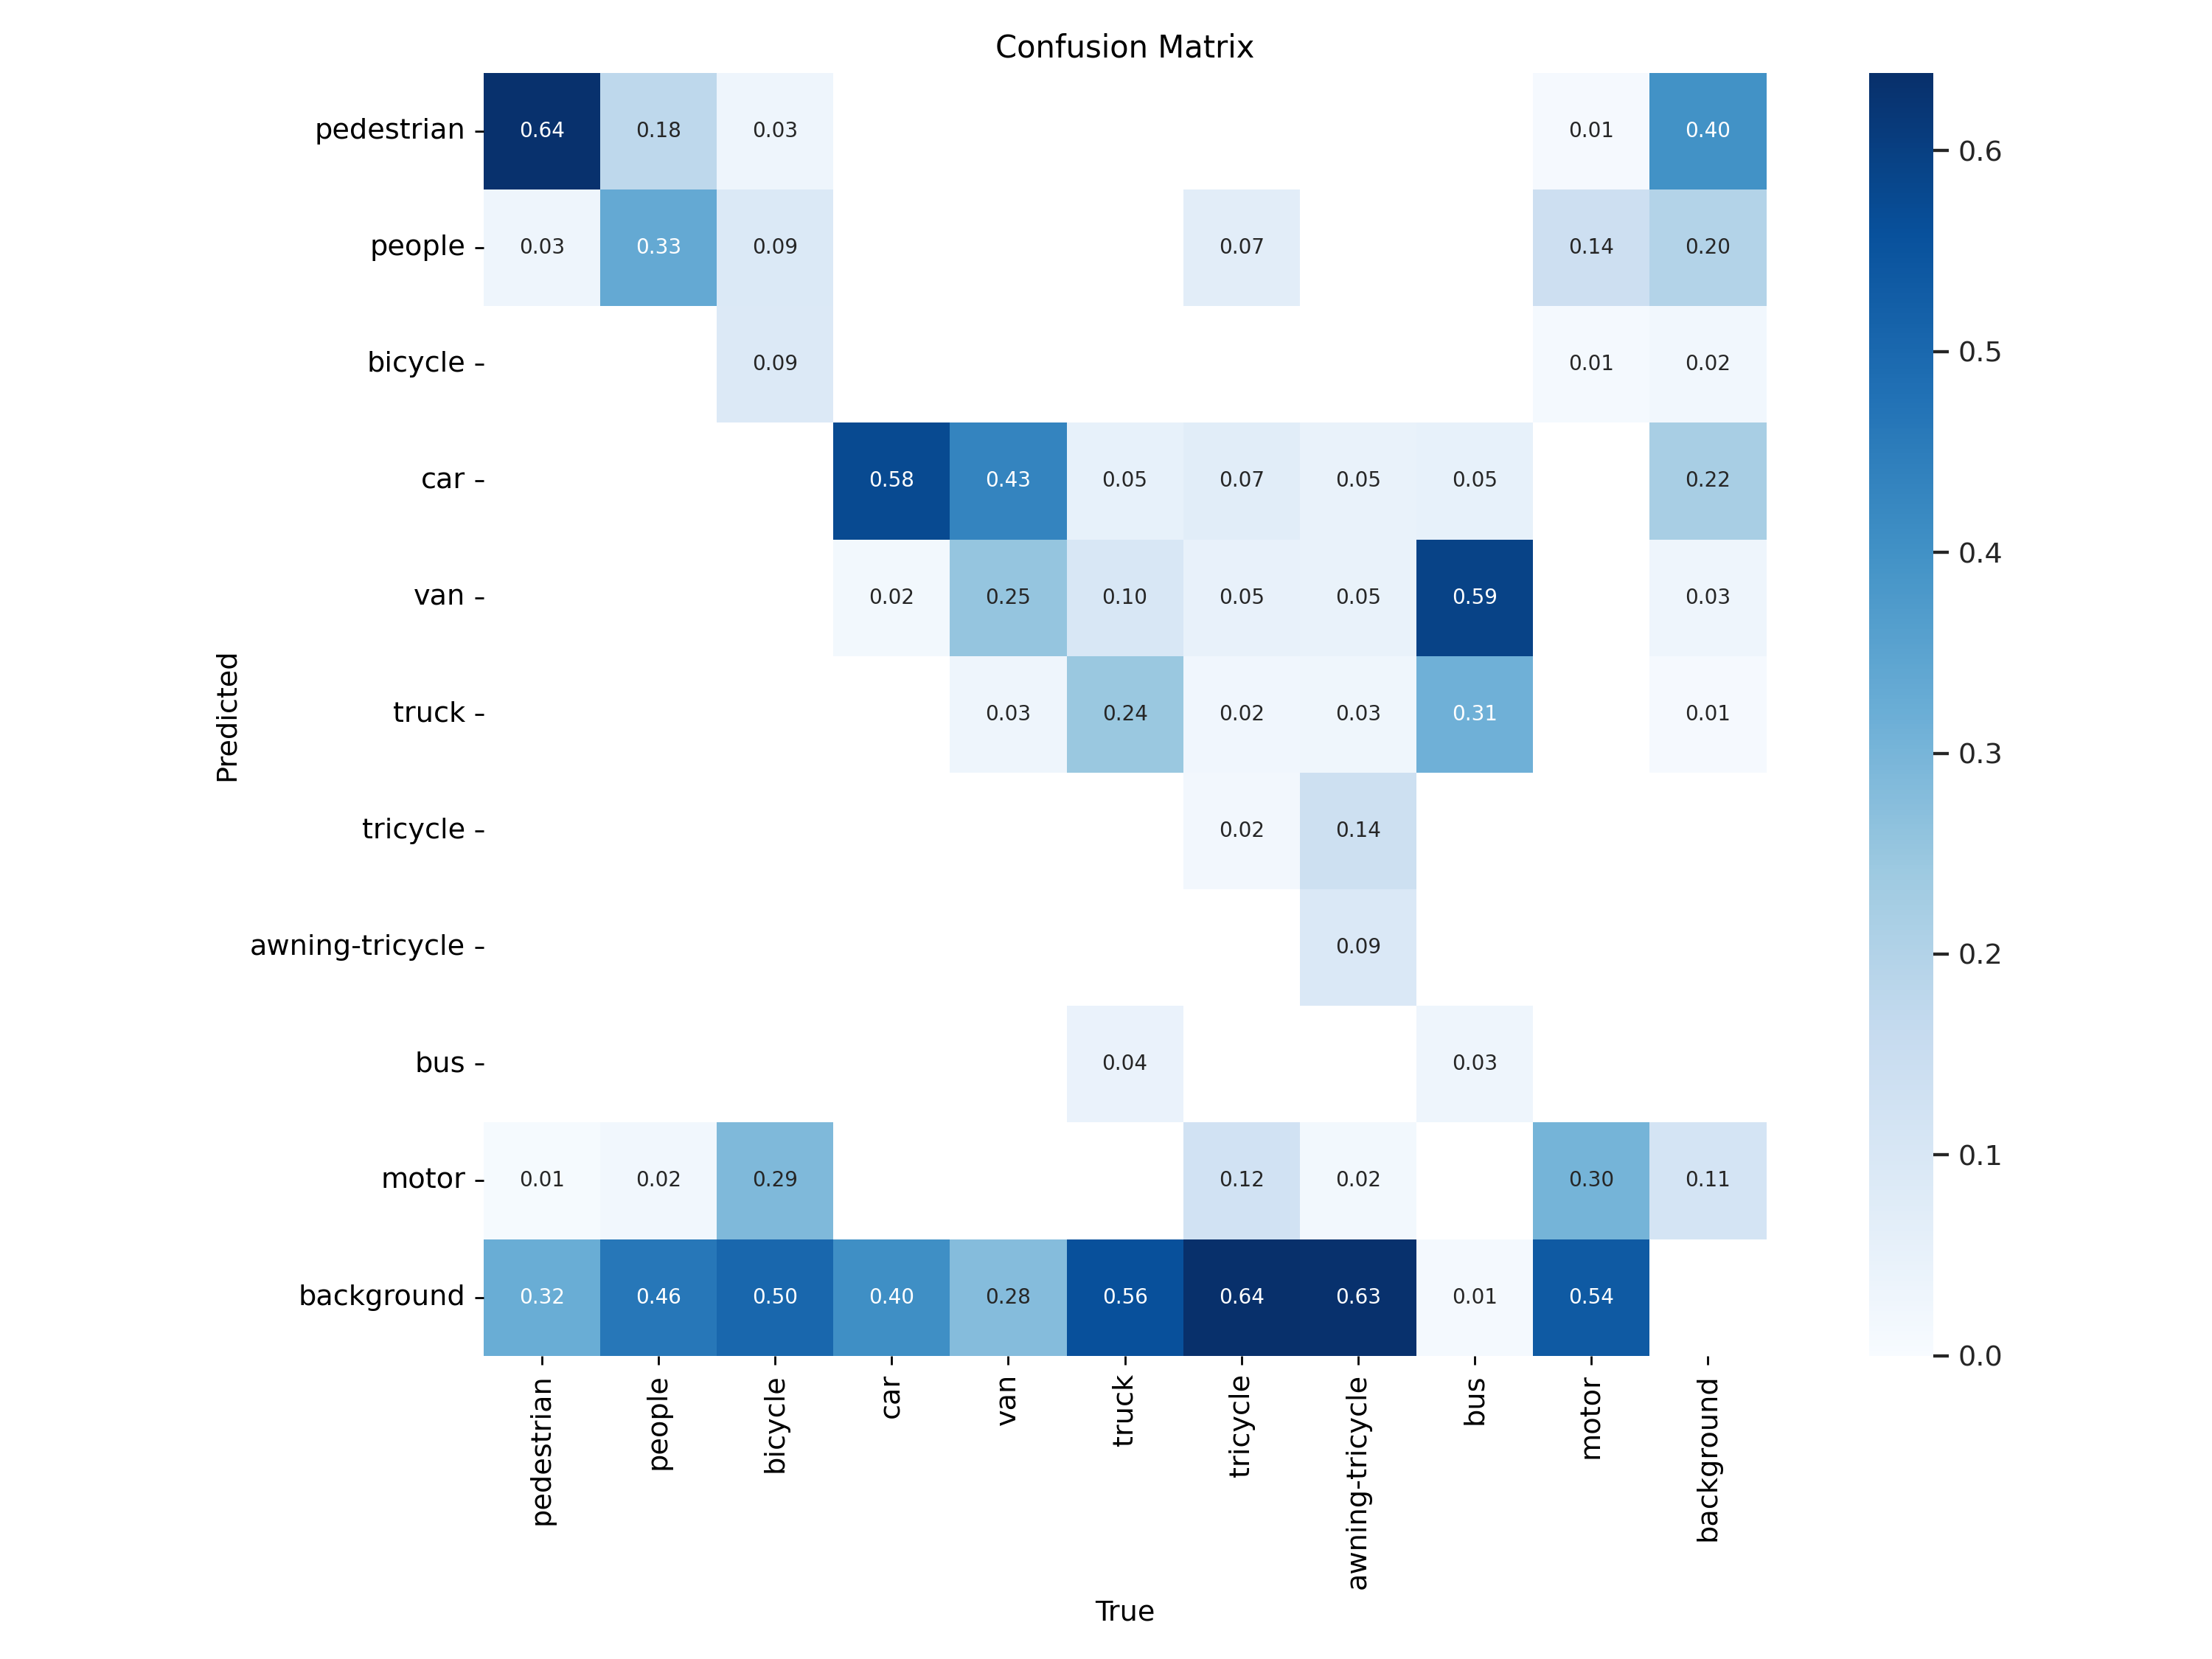
\includegraphics[width=0.85\textwidth]{10-2}
    \caption{Confusion Matrix после первого этапа обучения}
    \label{img:10-2}
\end{figure}

С целью решения первой из вышеприведенных проблем была поставлена задача улучшения датасета, для чего была проведена описанная ранее в работе обработка данных датасета VisDrone, состоящая из аугментации на этапе подготовки данных. После чего было проведено дополнительное обучение длительностью в 100 эпох более крупной модели YOLOv5x, в результате которого $mAP$ повысился до $45.6$, благодаря более высоким результатам на ранее малопредставленных классах, что видно на Рис. \ref{img:10-3}.

\begin{figure}[ht]
    \centering
    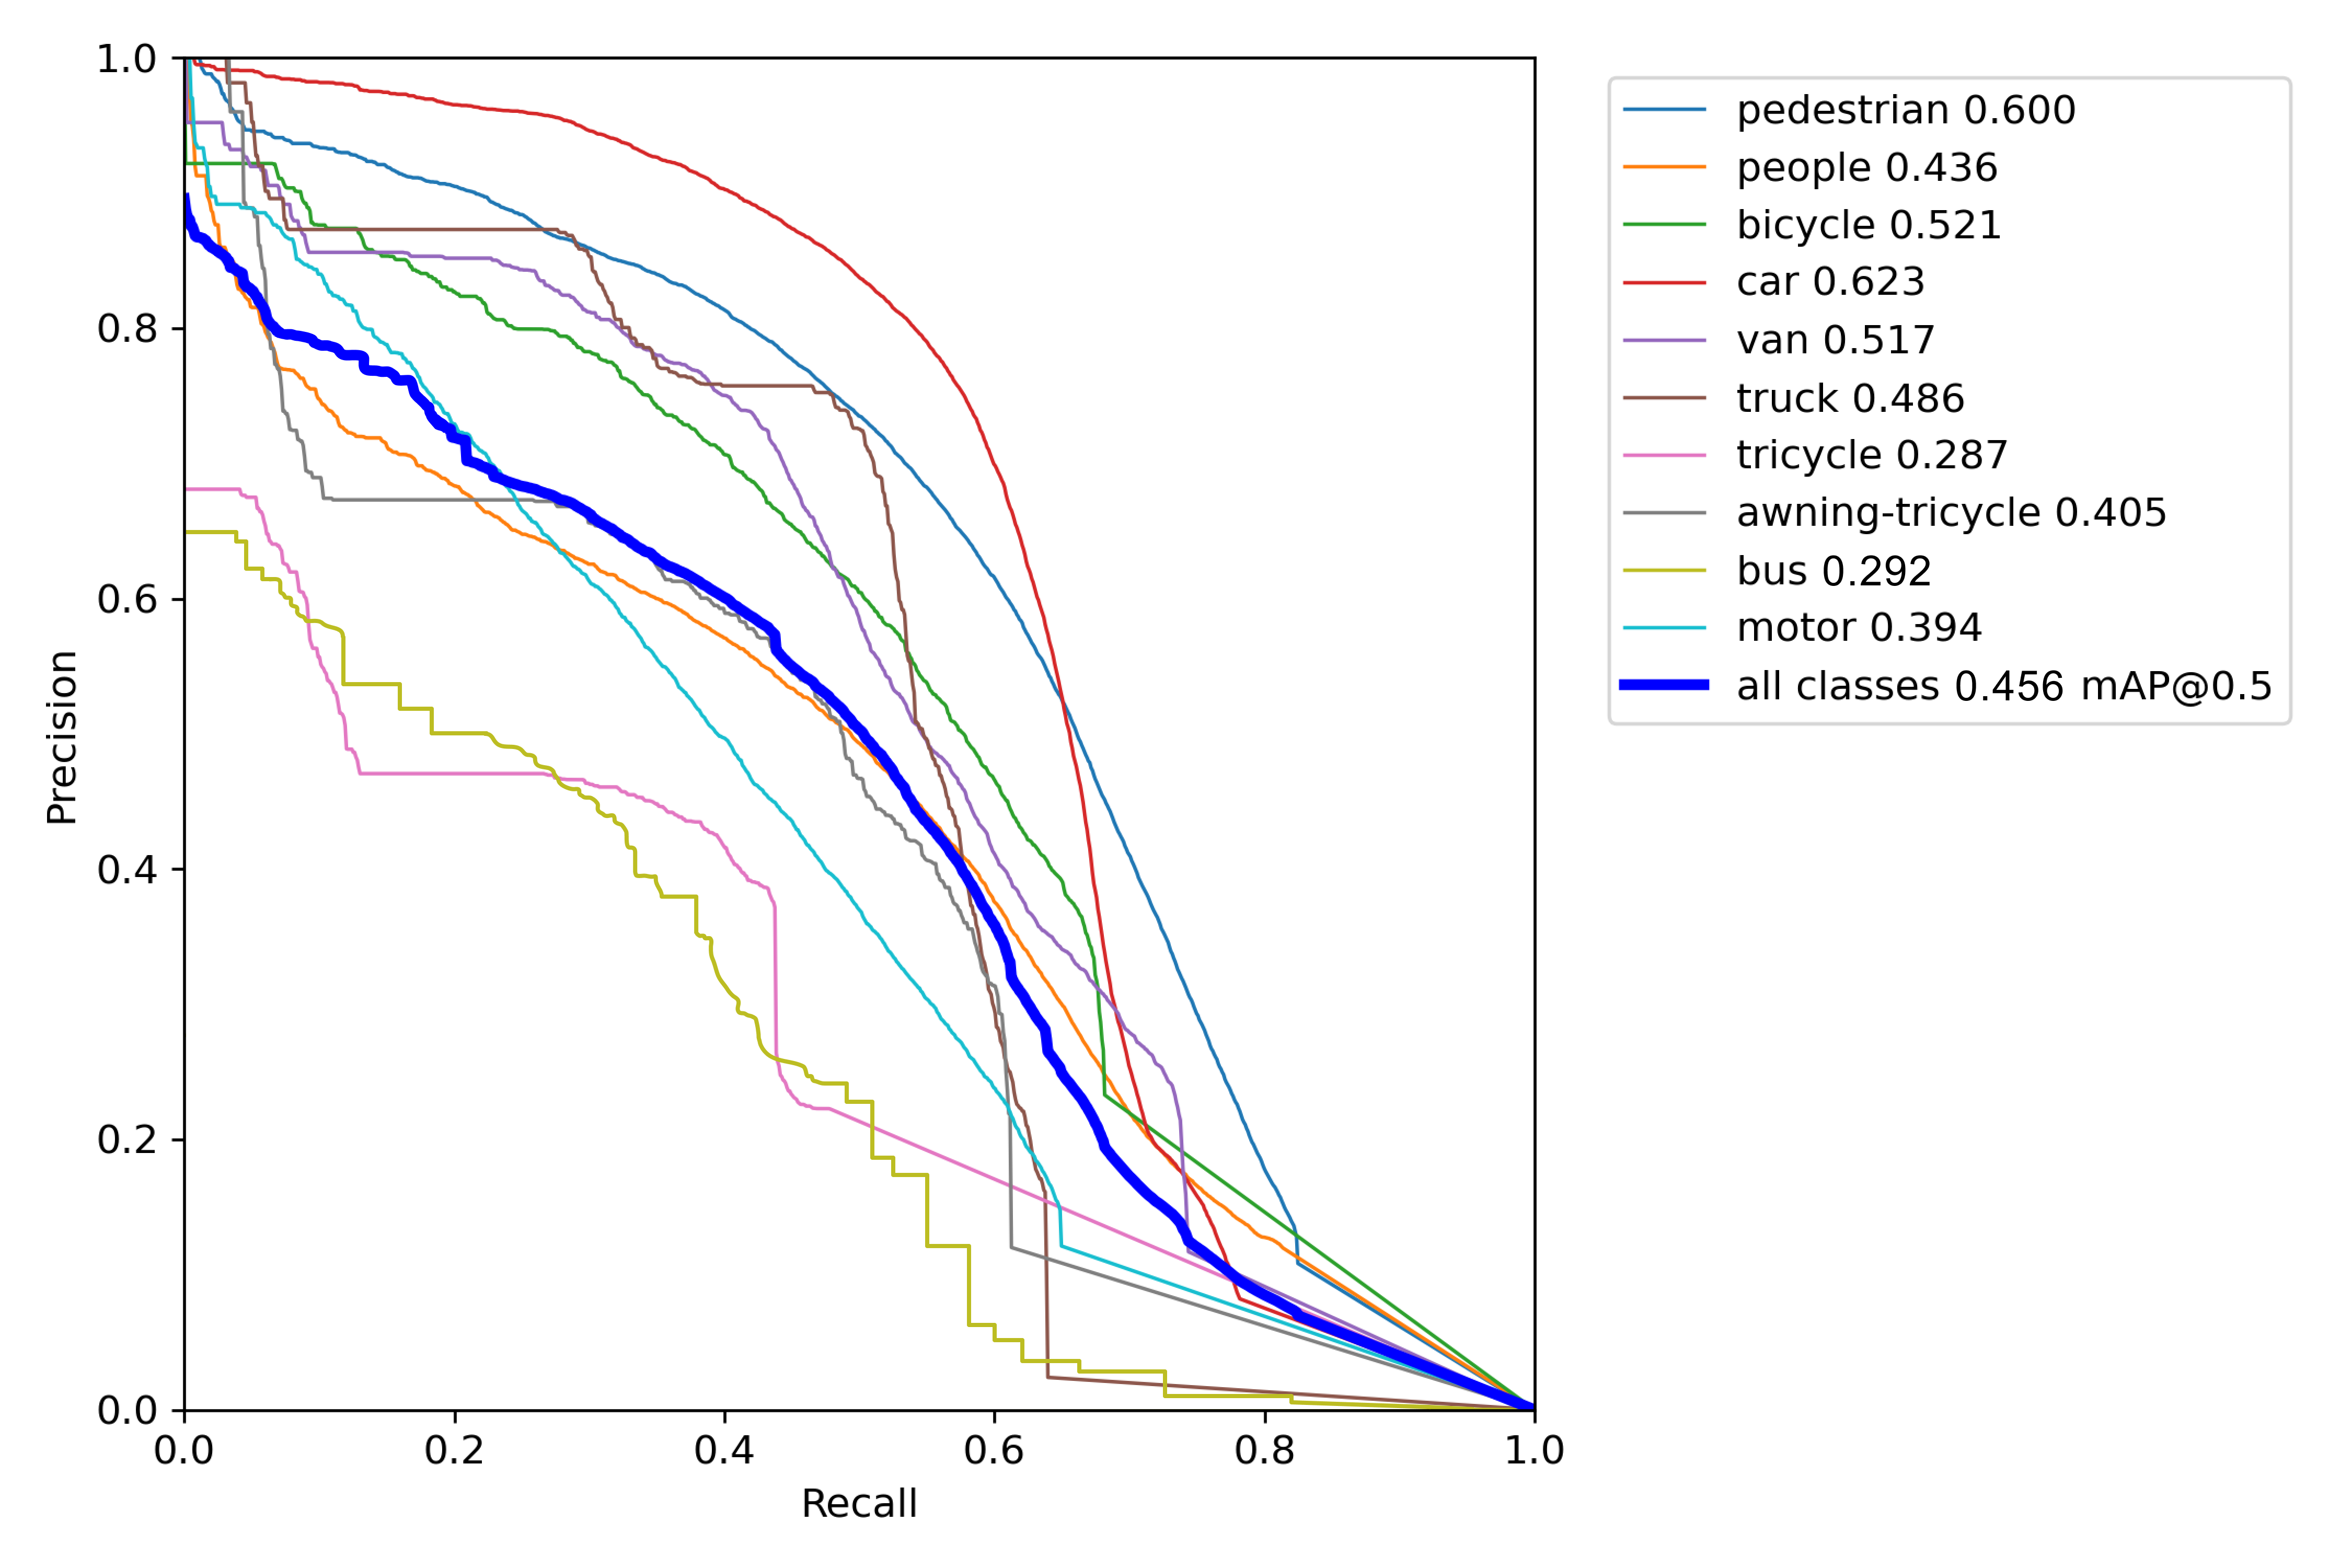
\includegraphics[width=0.85\textwidth]{10-3}
    \caption{Precision-Recall Curve после второго этапа обучения}
    \label{img:10-3}
\end{figure}

Для работы со второй проблемой из вышеуказанных были выполнены подготовка аннотаций для датасета UAVDT, отбор по результатам анализа подходящих видеопоследовательностей из него, содержащих сценарии расположения объектов вдалеке и в плотных скоплениях, а также дообучение длительностью в 50 эпох предыдущей модели, показавшее $mAP \ 48.1$, как на Рис. \ref{img:10-4}.

\vspace{0.5cm}

\begin{figure}[ht]
    \centering
    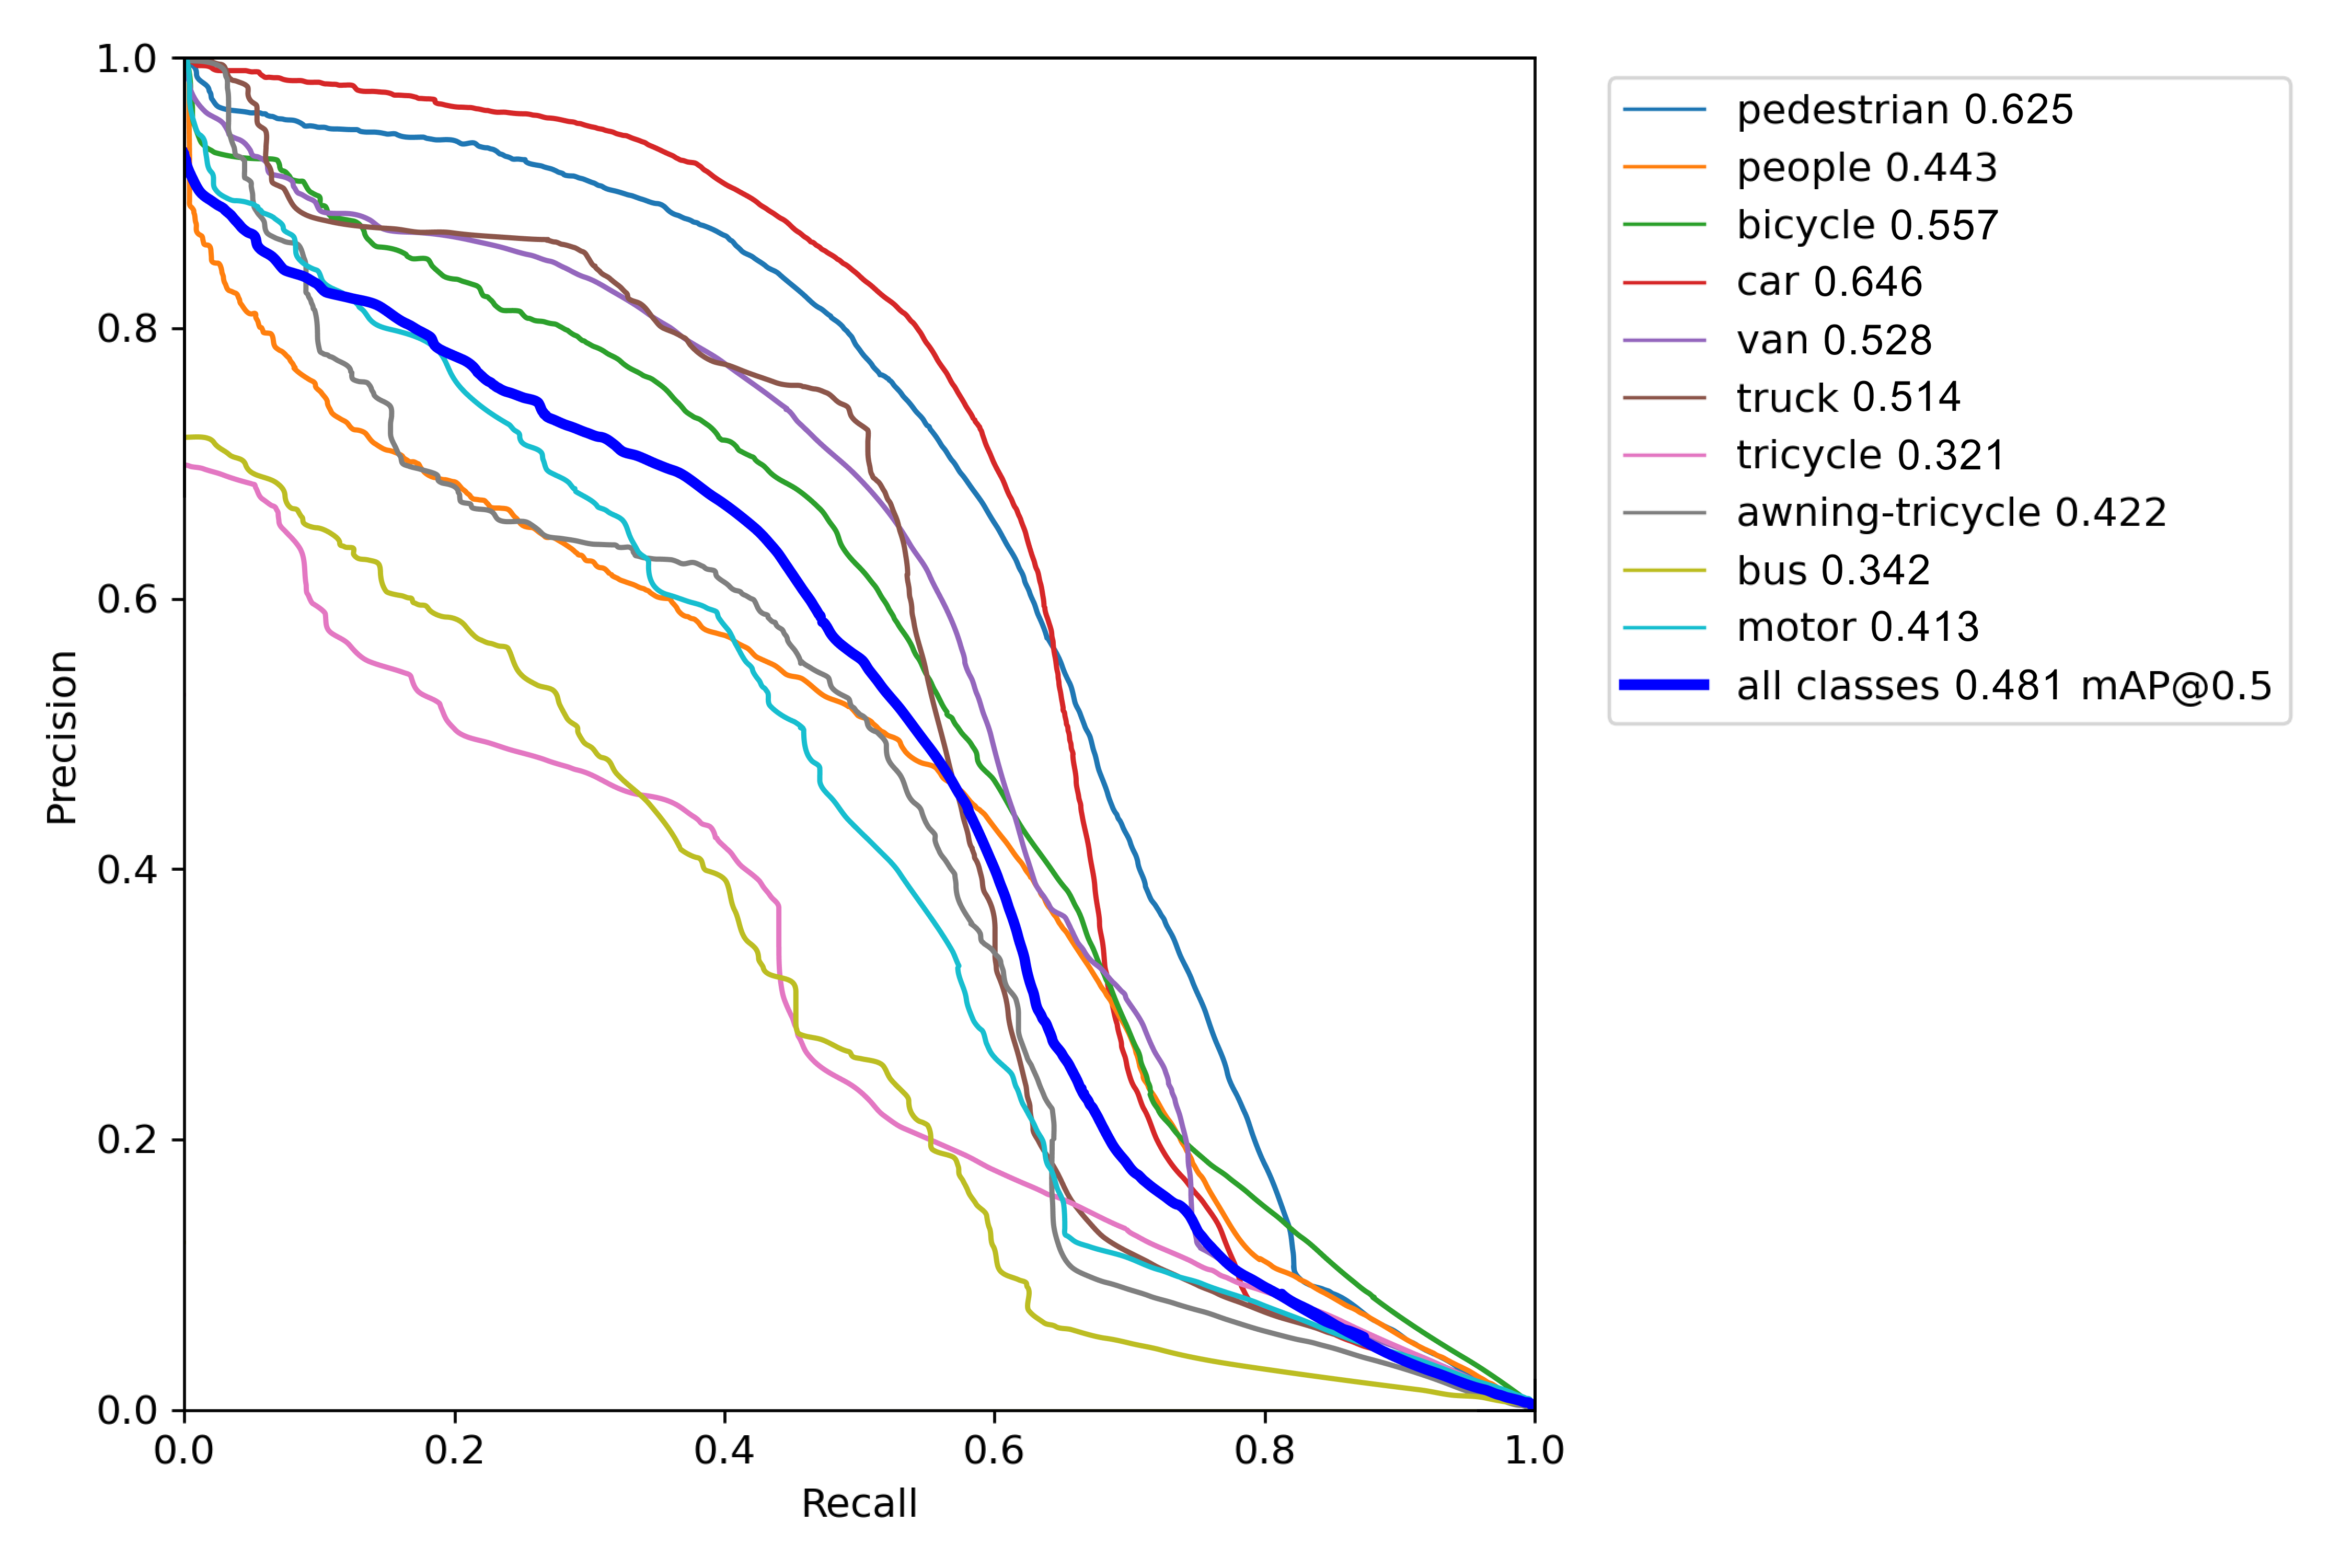
\includegraphics[width=0.85\textwidth]{10-4}
    \caption{Precision-Recall Curve после третьего этапа обучения}
    \label{img:10-4}
\end{figure}

В Таблице \ref{tbl:10-1} представлены результаты обучения на каждом этапе, показавшие значительное улучшение в точности благодаря обработке датасета VisDrone и дообучению на сложных сценариях из датасета UAVDT.

\vspace{0.5cm}

\begin{table}[ht]
    \centering
    \begin{tblr}{c|c}
        \hline[1.5pt]
        Этап & $mAP$ \\
        \hline[1.5pt]
        Без аугментаций & 30.0 \\
        \hline
        Обработка VisDrone & 45.6 \\
        \hline
        Обработка VisDrone + UAVDT & 48.1 \\
        \hline[1.5pt]
    \end{tblr}
    \caption{Результаты на этапе покадрового детектирования}
    \label{tbl:10-1}
\end{table}
